\question
(0,5 балла) Паркурщик Гамильтон и мотоциклист Эйлер участвуют в гонках по городу: Гамильтон бежит по крышам вдоль улиц, а Эйлер гоняет по улицам на своём мотоцикле.

\begin{minipage}[h]{0.45\linewidth}
\center{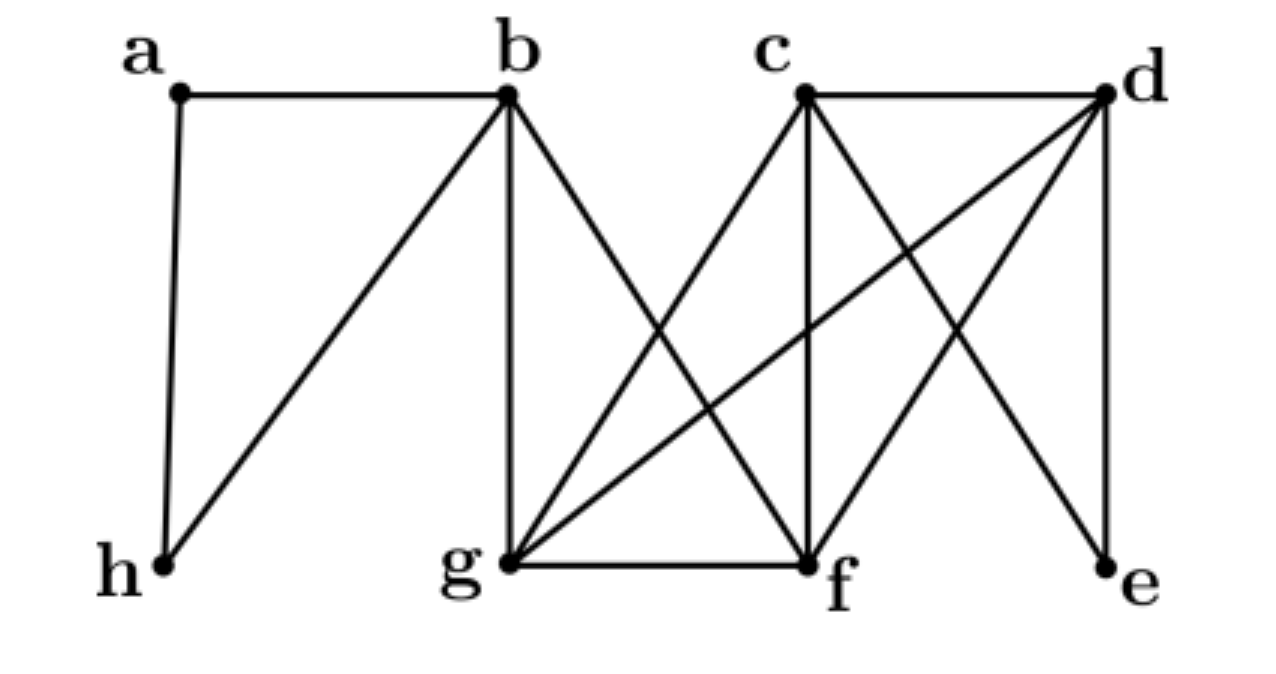
\includegraphics[width=0.7\textwidth]{pic/87.png} }
\end{minipage}

\begin{itemize}
\item Сможет ли Эйлер хотя бы закончить эту гонку? (Есть ли в графе Эйлеров цикл или Эйлерова цепь? Если есть, то постройте по шагам алгоритма Флери цепь/цикл. Если нет, то обоснуйте отсутствие)
\item Сможет ли Гамильтон хотя бы закончить эту гонку? (Есть ли в графе Гамильтонов цикл, Гамильтонова цепь? Если есть, постройте по шагам алгоритма цепь/цикл. Если нет, то обоснуйте отсутствие (проверьте все теоремы))
\item Преобразуйте граф, добавляя новые рёбра и/или вершины, чтобы он был одновременно и Гамильтоновым, и Эйлеровым, и гонка была честной.
\end{itemize}
